% Generated from: Zhihu/专栏：概率与统计/泛函中心极限定理：从 Brown 运动到 α‑稳定过程_金鱼马_2026-04-09.md
\section{基本概念和准备}

\subsection{两种随机函数的构造}

如何把 $S_n$ ``视作随机函数''呢？具体来说，我们要做的是将其视作 $[0,1]$ 上的连续时间随机过程 $S_n(\cdot)$。这便需要对时间轴和空间尺度同时进行变换。

最简单的做法是，在离散时间点 $t = k/n$（$k = 0,1,\dots,n$）处，定义
\[S_n\Bigl(\frac{k}{n}\Bigr) = \frac{1}{\sigma\sqrt{n}} \bigl( S_k - \mu k \bigr).\]
然后，对于任意的 $t \in [0,1]$，用直线接相邻的点 $(k/n, S_n(k/n))$ 和 $((k+1)/n, S_n((k+1)/n))$。显式写出来就是
\[S_n(t)=\frac{1}{\sigma\sqrt{n}}  \Bigl(S_{[nt]}-\mu [nt]+(nt-[nt])(X_{[nt]+1}-\mu)\Bigr)\]
其中 $[nt]$ 表示 $nt$ 的整数部分。这样得到的 $S_n(t)$ 是一个连续的折线函数，其样本路径属于连续函数空间 $\mathcal{C}[0,1]$。换言之，$S_n$ 定义了一个从概率空间到连续函数空间的随机变量（或者称随机函数）：
\[\begin{array}{ccl} S_n: & (\Omega,\mathscr F, P)&\to \mathcal C[0,1]\\ & \omega &\mapsto  S_n(\cdot,\omega) \end{array}\]
我们称 $\{S_n(t)\}_{n=1}^\infty$ 是由随机变量 $\{X_n\}_{n=1}^\infty$ 产生的\emph{部分和过程序列}。

传统中心极限定理的目标是考察部分和 $S_n$ 在 $(\mathbb R,\mathcal B_{\mathbb R})$ 中的弱收敛性；而面对部分和过程序列 $\{S_n(t)\}_{n=1}^\infty$，我们的目标便是研究它在 $\mathcal C[0,1]$ 中的弱收敛性。注意，这里我们要为连续函数空间 $\mathcal C[0,1]$赋予上确界范数
\[\|x\|_\infty = \sup_{0\le t\le 1}|x(t)|\]
及其生成的 Borel $\sigma$-代数 $\mathscr C$ ；此时在度量 \[ \rho(x,y):=\|x-y\|_\infty=\sup\limits_{0\le t\le 1}|x(t)-y(t)| \]下的收敛对应了一致收敛，称 $\rho$ 为一致收敛度量，其诱导的拓扑为一致收敛拓扑。

另一种更简单的构造是
\[\widetilde S_n(t) = \frac{1}{\sigma\sqrt{n}} \bigl( S_{[nt]} - \mu [nt] \bigr), \qquad 0 \le t \le 1,\]
这个函数在区间 $[k/n, (k+1)/n)$ 上为常数，在 $t = k/n$ 处可能有跳跃。因此它的样本路径是\emph{右连左极}的。

\begin{definition*}[右连左极函数]
设 $(M,d)$ 是度量空间，$E\subset\mathbb R$。若函数 $f:E\to M$ 满足：

\begin{itemize}
\tightlist
\item
  右连续：$f(t+)=\lim\limits_{s\to t^+} f(s)$ 存在，且等于 $f(t)$;
\item
  左极限：$f(t-)=\lim\limits_{s\to t^-} f(s)$ 存在且有限。
\end{itemize}

那么称 $f$ 是``右连续且存在左极限'' 的，简称``\textbf{\emph{右连左极}}''。法文称为 \textbf{\emph{\href{https://en.wikipedia.org/wiki/C\%C3\%A0dl\%C3\%A0g}{Càdlàg}}} （continue à droite, limite à gauche）。
\end{definition*}

我们将 $[0,1]$ 上全体``右连左极''的实值函数构成的集合记作 $\mathcal D[0,1]$。显然

\begin{itemize}
\tightlist
\item
  $\mathcal D[0,1]$ 中所有函数的间断点都是第一类间断点；
\item
  $\mathcal D[0,1]\supset \mathcal C[0,1]$ 。
\end{itemize}

同样在 $\mathcal D[0,1]$ 中赋予上确界范数及其生成的 Borel $\sigma$-代数。

显然，$\widetilde S_n(t)$ 与 $S_n(t)$ 在分点 $k/n$ 处取值相同，但前者是阶梯函数，后者是折线。当 $n$ 很大时，两者在视觉上非常接近，直觉上二者应该有同样的收敛性结论。

\subsection{Brown 运动}

\begin{definition*}[标准 Brown 运动]
$[0,1]$ 上的实值随机过程 $B(t)$ 如果满足以下四个条件：

\begin{enumerate}
\def\labelenumi{\arabic{enumi}.}
\tightlist
\item
  \emph{起点为零}：$B(0) = 0$ a.s.。
\item
  \emph{独立增量}：对任意 $0 \le t_0 < t_1 < \dots < t_m \le 1$，增量 $B(t_1)-B(t_0), \dots, B(t_m)-B(t_{m-1})$ 相互独立。
\item
  \emph{增量正态性}：对每个 $s,t \in [0,1]$，$t\ge s$，$B(t)-B(s) \sim N(0, t-s)$。
\item
  \emph{路径连续性}：样本路径 $t \mapsto B(t)$ a.s. 连续。
\end{enumerate}

则称 $B(t)$ 为标准 \textbf{\emph{\href{https://en.wikipedia.org/wiki/Brownian_motion}{Brown 运动}}} （或 Wiener 过程）。它也可以视作将概率空间 (a.s. 地) 映射到 $\mathcal C[0,1]$ 的随机函数：
\[\begin{array}{ccl} B: & (\Omega,\mathscr F, P)&\to \mathcal C[0,1]\\ & \omega &\mapsto  B(\cdot,\omega) \end{array}\]\end{definition*}

图~\ref{fig:e2:brownian-paths} 展示了标准 Brown 运动的若干条样本轨迹。

\begin{figure}[htbp]
  \centering
  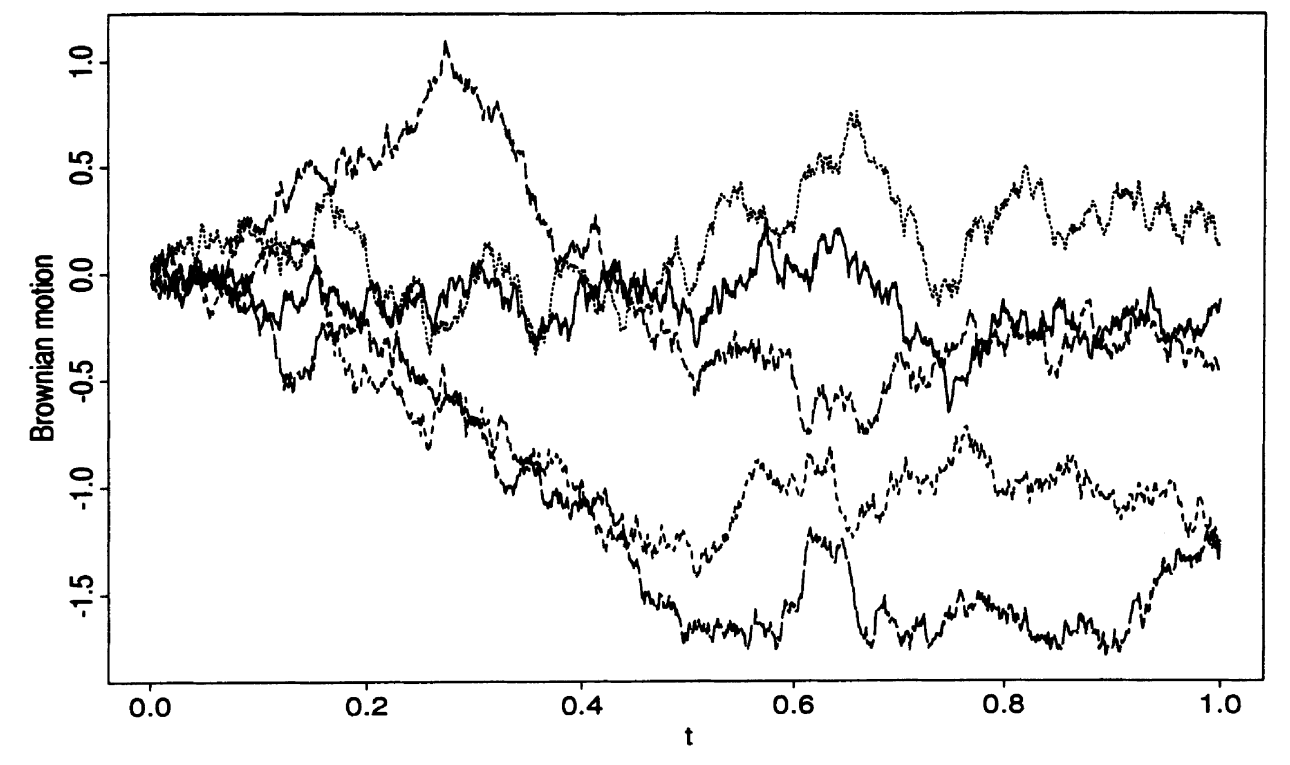
\includegraphics[width=0.88\textwidth]{figures/e2-brownian-paths.png}
  \caption{$[0,1]$ 上标准 Brown 运动的五条样本轨迹。图片来自 \cite{embrechts1997}, p.~89}
  \label{fig:e2:brownian-paths}
\end{figure}

Brown 运动是概率论中最重要的随机过程之一，其存在性和构造、以及相关的性质（样本路径 Hölder 连续、几乎处处不可微、变差无界等等）和理论等，我们在此不必多提，随便一本教材上都会讲解。在这里，我们要用标准 Brown 运动替代经典中心极限定理中的正态分布 $\mathcal N(0,1)$，扮演``极限过程''的核心角色。

\subsection{度量空间中的弱收敛}

回顾弱收敛的定义~\ref{def:ch1:weak-convergence}：设 $(S, \rho)$ 是一个度量空间（$\rho$ 是距离函数），并赋予其 Borel $\sigma$-代数（由所有开集生成）。令 $X, X_1, X_2, \dots$ 是取值于 $S$ 的随机元。如果对任意有界、连续的实值函数 $f: S \to \mathbb{R}$，都有
\[\lim_{n\to\infty}\mathbb{E}[f(X_n)]=\mathbb{E}[f(X)]\]
称序列 ${X_n}$ 弱收敛 于 $X$（记作 $X_n \overset{\rm d}\to X$）。当 $S = \mathbb{R}$ 且 $\rho$ 是通常绝对值距离时，上述定义就退化为经典的随机变量弱收敛，即，依分布收敛。
当然，我们面临的空间 $S$ 是 $\mathcal C[0,1]$ 或者 $\mathcal D[0,1]$ ，在证明依分布收敛时，上面这个``用有界连续函数刻画''的标准定义总是不太方便。更具有操作性的框架是借助 Prokhorov 定理（定理~\ref{thm:ch1:prohorov}），将弱收敛拆解为``有限维分布的收敛''加上``相对紧性（由一致胎紧性保证）''。
% \begin{definition*}[胎紧]
% 取值于度量空间 $S$ 上的一族随机变量 $\{X_\pi\}_{\pi\in\Pi}$ 如果满足：对任意 $\epsilon>0$，有紧集 $K\subset S$，使得 $\sup\limits_{\pi\in\Pi}P(X_\pi\notin K)<\epsilon$，则称这族随机变量是\textbf{\emph{胎紧}} (tight) 的。简而言之，胎紧意味着一族随机变量一致地集中在一个紧集上。
% \end{definition*}
% \begin{theorem}[Prokhorov 定理]
% \label{thm:ext-fclt:prokhorov}
% 若取值于度量空间 $S$ 上的一族随机变量 $\{X_\pi\}_{\pi\in\Pi}$ 是一致胎紧的，则其是 (弱) \textbf{\emph{相对紧}} 的，即，其中的任意序列 $\{X_{n}\}_{n=1}^\infty$ 有弱收敛的子列。反过来，若 $S$ 是可分完备度量空间，那么 $S$ 上的概率测度族相对紧蕴含一致列紧。
% \end{theorem}
在 $(\mathcal C[0,1],\rho)$ 中，有限维柱集构成了\emph{确定类} (determining class / separating class)。简而言之，这是说，对于取值于 $\mathcal C[0,1]$ 的随机元，如果我们能确定它的所有有限维分布，即，对任意 $0\le t_1<\cdots<t_m\le 1$ ，我们能确定 $(X(t_1),\dots,X(t_m))$ 的分布，就可以确定 $X$ 本身的分布 (e.g., 见 \url{https://math.stackexchange.com/q/3450060})；这一结论单独还不足以确定收敛性，但只要与 Prokhorov 定理结合起来，便能得到

\begin{corollary}\label{cor:ext-fclt:finite-dimensional-tightness}
设 $X_n$ 和 $X$ 是取值于 $(\mathcal C[0,1],\rho)$ 的随机变量，$X_n\overset{\rm d}\to X$ 当且仅当如下两个条件成立：

\begin{itemize}
\tightlist
\item
  $\{X_n\}_{n=1}^\infty$ 一致胎紧；
\item
  对任意 $0\le t_1<\cdots<t_m\le 1$ ，有 $(X_n(t_1),\dots,X_n(t_m))\overset{\rm d}\to (X(t_1),\dots,X(t_m))$ 。
\end{itemize}
\end{corollary}

这个结论对后文要介绍到的 Skorokhod 度量 $(\mathcal D[0,1],d_0)$ 也是成立的。

\section{Donsker 定理}

所谓``泛函中心极限定理 (FCLT)''，确切来说叫 \textbf{\emph{Donsker 定理}} ，得名于 Monroe D. Donsker。其叙述如下：

\begin{theorem}

Donsker 定理：设 $X_1, X_2, \dots$ i.i.d.，$\mathbb{E}[X_1] = \mu$，$0 < \mathrm{Var}[X_1] = \sigma^2 < \infty$。则

\begin{itemize}
\tightlist
\item
  在 $(\mathcal{C}[0,1],\rho)$ 中，有 \[S_n(\cdot) \overset{\rm d}\to B({\cdot})\]\item
  在 $(\mathcal{D}[0,1],\rho)$ 中，有 \[\widetilde S_n(\cdot) \overset{\rm d}\to B(\cdot)\]\end{itemize}
\end{theorem}

该定理又称``Donsker 不变原理''，强调了极限过程与 $X_n$ 的具体分布无关 ------ 只要方差有限，其随机游走路径总是收敛到 Brown 运动。它是一个非常强大的结果。

我们这里不具体介绍其证明（因为比较繁琐）。非常简略来说，完整的证明需要两大部分：

\begin{enumerate}
\def\labelenumi{\arabic{enumi}.}
\tightlist
\item
  有限维分布收敛：对任意 $0 \le t_1 < \dots < t_m \le 1$，向量 $(S_n(t_1), \dots, S_n(t_m))$ 依分布收敛到 $(B(t_1), \dots, B(t_m))$。这需要用到独立增量性质。
\item
  胎紧性：证明序列 $\{S_n(\cdot)\}$ 在 $\mathcal{C}[0,1]$ 中是胎紧的。通常需要验证 \emph{一致连续性模} 的收敛：对任意 $\epsilon > 0$，
  \[
  \lim_{\delta \to 0} \limsup_{n\to\infty} P\Bigl( \sup_{|t-s|<\delta} |S_n(t)-S_n(s)| > \epsilon \Bigr) = 0.
  \]
\end{enumerate}

那么由上节推论，这两个条件等价于弱收敛。这个是 Billingsley 的经典证明。至于 $(\mathcal{D}[0,1],\rho)$ 的情形，证明要借助后文将介绍的 Skorokhod 拓扑。

图~\ref{fig:e2:donsker-convergence} 是 Donsker 定理的示意图。可以看到，随着 $n$ 逐渐增加， $S_n(\cdot)$ 越来越趋近于 Brown 运动的样本路径。

\begin{figure}[htbp]
  \centering
  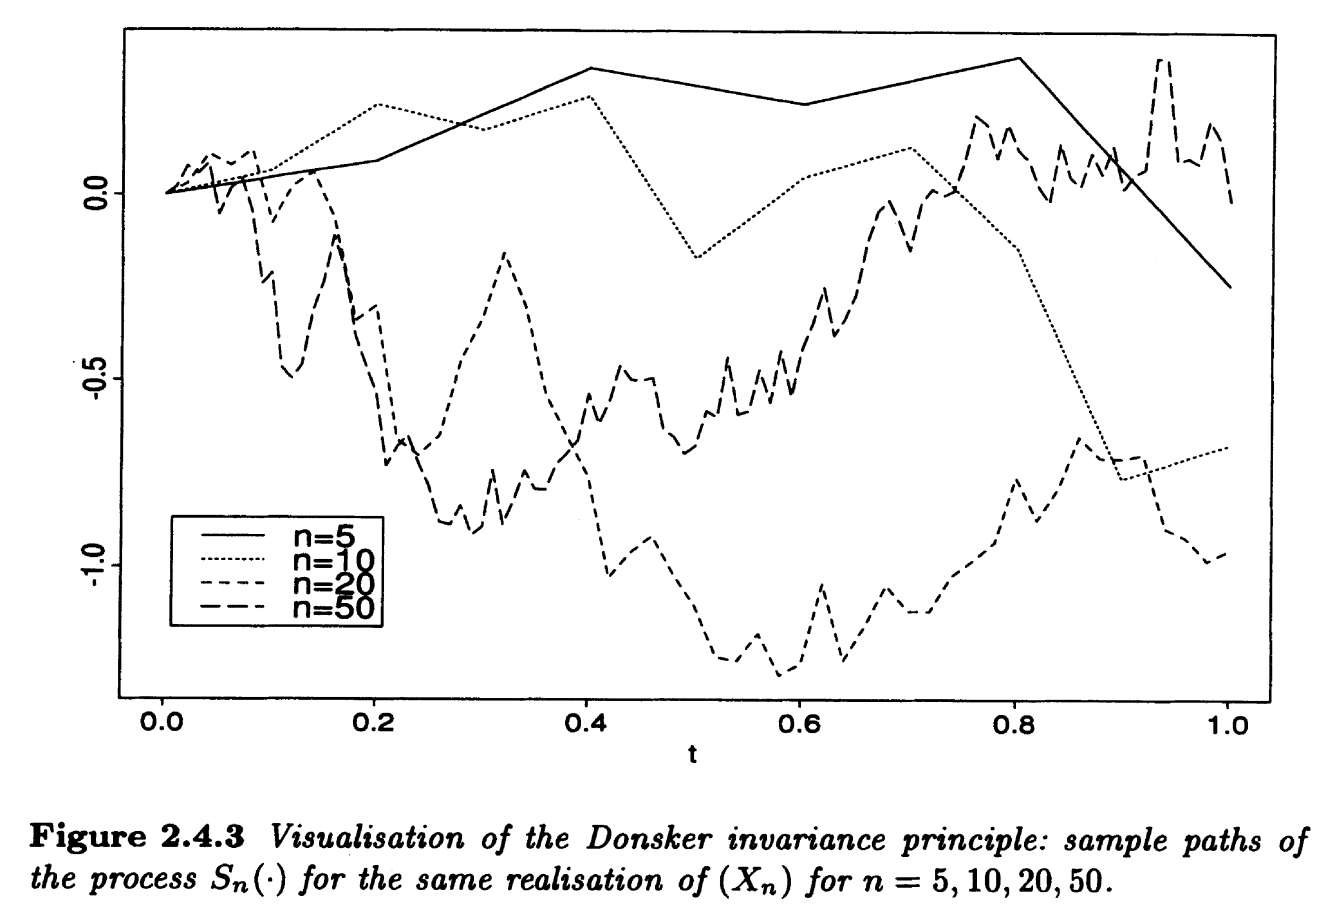
\includegraphics[width=0.88\textwidth]{figures/e2-donsker-convergence.png}
  \caption{Donsker 定理的示意图。图片来自 \cite{embrechts1997}, p.~90}
  \label{fig:e2:donsker-convergence}
\end{figure}

Donsker 定理可以配合连续映射定理 (定理~\ref{thm:ch1:continuous-mapping}) 来使用：


在 $\mathcal{C}[0,1]$ 或 $\mathcal{D}[0,1]$ 上，以下泛函在 $\rho$ 下是连续的：

\begin{itemize}
\tightlist
\item
  取值泛函：$f_1(x) = x(1)$。
\item
  最大值：$f_2(x) = \sup_{0\le t\le 1} x(t)$。
\item
  最小值：$f_3(x) = \inf_{0\le t\le 1} x(t)$。
\item
  振幅：$f_4(x) = \sup_t x(t) - \inf_t x(t)$。
\item
  积分：$f_5(x) = \int_0^1 x(t)\,\mathrm dt$。
\end{itemize}

利用 Donsker 定理和连续映射定理，我们立刻得到许多有用的收敛结果。

\begin{example}[Donsker 定理的连续泛函]
以 $f_1$、$f_2$、$f_3$ 为例，注意到
\[
\begin{aligned}
f_1(S(\cdot))=f_1(\widetilde S(\cdot))
  &=\frac{S_n-n\mu}{\sigma\sqrt n},\\
f_2(S(\cdot))=f_2(\widetilde S(\cdot))
  &=\frac1{\sigma\sqrt n}\max_{0\le k\le n}(S_k-k\mu),\\
f_3(S(\cdot))=f_3(\widetilde S(\cdot))
  &=\frac1{\sigma\sqrt n}\min_{0\le k\le n}(S_k-k\mu).
\end{aligned}
\]
那么
\[\begin{aligned} \frac{1}{\sigma\sqrt{n}} (S_n - n\mu) &\overset{\rm d}\to B(1)\overset{\rm d}=\mathcal N(0,1)\\ \frac{1}{\sigma\sqrt{n}} \max_{0\le k\le n} (S_k - k\mu) &\overset{\rm d}\to \sup_{0\le t\le 1} B(t)\\ \frac{1}{\sigma\sqrt{n}} \min_{0\le k\le n} (S_k - k\mu) &\overset{\rm d}\to \inf_{0\le t\le 1} B(t) \end{aligned}\]
更一般地，联合分布也收敛：
\[\Bigl( \frac{S_n - n\mu}{\sigma\sqrt{n}},\; \frac{\max_{k}(S_k - k\mu)}{\sigma\sqrt{n}},\; \frac{\min_{k}(S_k - k\mu)}{\sigma\sqrt{n}} \Bigr) \overset{\rm d}\to \bigl( B_1,\; \sup B(t),\; \inf B(t) \bigr)\]
\end{example}

\begin{example}[有限维分布]
取 $0\le t_1<\dots<t_m\le 1$，考虑 $\mathcal C[0,1]$ 上的泛函 $x\mapsto (x(t_1),\dots,x(t_m))$。该映射在 $\mathcal C[0,1]$ 上处处连续，因此
\[\bigl( S_n(t_1),\dots,S_n(t_m) \bigr) \overset{\rm d}\to (B(t_1),\dots,B(t_m)).\]
这表明 Donsker 定理蕴含有限维分布的收敛。

\end{example}

\section{Skorokhod 拓扑}

我们知道，一致收敛度量 $\rho$ 定义了函数空间 $\mathcal C[0,1]$ 和 $\mathcal D[0,1]$ 上的``一致收敛拓扑''，在此拓扑下，两个函数 $x(t)$ 和 $y(t)$ ``很接近''，是指 $x(t)$ 的图像可以经过纵坐标的一个一致小的移动得到 $y(t)$。这个条件是比较强的，例如，假设有两个阶梯函数 $x(t) = \mathbf{1}_{[0.5, 1]}(t)$ 和 $y(t) = \mathbf{1}_{[0.5+\epsilon, 1]}(t)$。它们都只有一个跳跃点，且跳跃时间仅仅相差 $\epsilon$。从直觉上看，当 $\epsilon$ 极小时，这两个路径应该是``极度相似''的。但是，如果用一致收敛度量，$\rho(x,y) = \sup_t |x(t)-y(t)| \equiv 1$。这意味着无论 $\epsilon$ 多小，它们在一致拓扑下都无法靠近。

于是，我们希望能放宽一致收敛的条件，允许横坐标（时间尺度）也可以有一个一致小的变动。Skorokhod 拓扑就体现了这一想法。

由于 α-稳定运动（$\alpha<2$）的路径有跳跃，我们不能在 $\mathcal{C}[0,1]$ 中处理，因此需要在 $\mathcal D[0,1]$ 上定义，

\begin{definition*}[Skorokhod $J_1$ 度量]
设 $\Lambda$ 为所有严格递增连续函数 $\lambda:[0,1]\to[0,1]$ 满足 $\lambda(0)=0,\lambda(1)=1$。对 $\mathcal D[0,1]$ 中任意两个元素 $x,y$，定义 $d_1(x,y)$ 为满足下述性质的 $\epsilon$ 的下确界：存在 $\lambda \in \Lambda$ 使得
\[\sup_{0\le t\le 1}|\lambda(t)-t|\le\epsilon,\quad \sup_{0\le t\le 1}|x(t)-y(\lambda(t))|\le\epsilon\]
换言之，
\[d_1(x,y):= \inf_{\lambda\in\Lambda} \max\left\{ \sup_{0\le t\le 1} |\lambda(t)-t|,\; \sup_{0\le t\le 1} |x(t)-y(\lambda(t))| \right\}\]
则可以证明 $d_1(x,y)$ 定义了 $\mathcal D[0,1]$ 中的一个度量，其诱导的拓扑称作 Skorokhod 拓扑或者 $J_1$ 拓扑。
\end{definition*}

由定义看出，在此拓扑下， $x_n \to x$ 的意义是：存在 $\lambda_n \in \Lambda$ 使得
\[\sup_{0\le t\le 1} |\lambda_n(t)-t| \to 0, \quad \sup_{0\le t\le 1} |x_n(t) - x(\lambda_n(t))| \to 0.\]
即允许在时间上做轻微拉伸/压缩，使函数值接近。

虽然度量 $d_1$ 本身不完备，但存在与之等价的完备度量 $d_0$，使得二者诱导的拓扑相同，因此 $d_0(x_n,x)\to 0$ 当且仅当 $d_1(x_n,x)\to 0$。

\begin{theorem}

取 $\Lambda$ 的子集 $\Lambda_0$：$\lambda\in\Lambda_0$ 当且仅当
\[\|\lambda\|_0:=\sup_{0\le s\ne t\le 1}\left|\log\frac{\lambda(t)-\lambda(s)}{t-s}\right|<\infty\]
定义 $d_0$ 为满足如下性质的 $\epsilon$ 的下确界：
\[\|\lambda\|_0\le\epsilon,\quad \sup_{0\le t\le 1}|x(t)-y(\lambda(t))|\le\epsilon\]
换言之，
\[d_0(x,y):=\inf_{\lambda\in\Lambda_0}\max\left\{\|\lambda\|_0,\,\sup_{0\le t\le 1}|x(t)-y(\lambda(t))|\right\}\]
则，$d_0$ 是一个和 $d_1$ 等价的度量，且 $(\mathcal D[0,1], d_0)$ 可分完备。


\end{theorem}
本文中 Skorokhod 度量（或者 $J_1$ 度量）总指的是 $d_0$ 。

相比于一致收敛度量
\[\rho(x,y)=\sup_{0\le t\le 1}|x(t)-y(t)|\]
可以证明 $(\mathcal D[0,1],\rho)$ 完备但不可分，且对任意 $x,y\in \mathcal D[0,1]$，$d_0(x,y)\le \rho (x,y)$，由此可见一致收敛拓扑比 Skorokhod 拓扑来得更加精细，$\rho(x_n,x)\to 0\implies d_0(x_n,x)\to 0$。但是，能证明：当 $x\in\mathcal C[0,1]$ 时，反过来也是成立的：$d_0(x_n, x)\to 0\implies \rho(x_n,x)\to 0$。

这立即得到如下结论，

\begin{theorem}

设 $[0,1]$ 上的随机过程 $Y_1,Y_2,\dots$ 的样本路径总是右连左极的（即，取值于 $\mathcal D[0,1]$），$Y$ 的样本路径依概率 1 在 $[0,1]$ 上连续（即，取值于 $\mathcal C[0,1]$）。那么，在 $(\mathcal D[0,1],d_0)$ 中，$Y_n\overset{\rm d}\to Y$，当且仅当在 $(\mathcal D[0,1],\rho)$ 中 $Y_n\overset{\rm d}\to Y$。

\end{theorem}

\begin{corollary}\label{cor:ext-fclt:donsker-skorokhod}
Donsker 定理对 $\mathcal D[0,1]$ 配备 Skorokhod 度量 $d_0$ 时成立（证明思路与 $(\mathcal C[0,1], \rho)$ 情形相同）。从而，根据上述定理，Donsker 定理对 $(\mathcal D[0,1],\rho)$ 成立。
\end{corollary}

(有关于 Skorokhod 拓扑的介绍性文章见 \cite{kern2023}。)

\section{α‑稳定过程}

经典 FCLT 要求方差有限，这意味着分布的尾部不能太厚。但在许多实际问题中，观测值往往表现出``尖峰重尾''特征，其方差甚至期望可能无穷大。例如，对\href{https://en.wikipedia.org/wiki/Power_law\#Power-law_probability_distributions}{幂律尾} (power-law tail) 的分布，即满足 $P(|X|>t)\propto t^{-\alpha}$ ，有广义中心极限定理 (GCLT) 成立，不过其部分和的归一化常数也不再是 $\sqrt{n}$，而是 $n^{1/\alpha}$，其中 $\alpha \in (0,2)$ 是所谓的\emph{尾指数} (tail index)。此时的极限分布也不再是正态，而是 \emph{\textbf{\href{https://en.wikipedia.org/wiki/Stable_distribution}{α‑稳定分布}} }。

% 请读者参考

% \hyperref[ext:stable-distributions]{扩展阅读《稳定分布》}

类似于 α-稳定分布的概念，我们可以将 Brown 运动进行推广。

\begin{definition*}[平稳独立增量与 Lévy 过程]
设 $\alpha\in(0,2]$。一个 $[0,1]$ 上的实值随机过程 $\xi(t)$ 称其满足

\begin{itemize}
\tightlist
\item
  \emph{独立增量} 性质：若对任意 $0 \le t_0 < t_1 < \dots < t_m \le 1$，增量 $\xi(t_1)-\xi(t_0), \dots, \xi(t_m)-\xi(t_{m-1})$ 相互独立。
\item
  \emph{平稳增量} 性质：若对任意 $s,t\in[0,1]$，$s<t$，有 $\xi(t)-\xi(s)\overset{\rm d}=\xi(t-s)$ 。
\end{itemize}

如果 $\xi(t)$ 满足平稳、独立增量性质，且样本路径总在 $\mathcal D[0,1]$ 中（右连左极），则称 $\xi(t)$ 是一个 \textbf{\emph{\href{https://en.wikipedia.org/wiki/L\%C3\%A9vy_process}{Lévy 过程}}} 。
\end{definition*}

\begin{definition*}[$\alpha$-稳定过程]
设 $\alpha \in (0,2]$。一个 $[0,1]$ 上的实值随机过程 $\xi(t)$ 如果满足：

\begin{enumerate}
\def\labelenumi{\arabic{enumi}.}
\tightlist
\item
  $\xi(0) = 0$ a.s.；
\item
  是 Lévy 过程，即：有平稳独立增量性质，样本路径总在 $\mathcal D[0,1]$ 中；
\item
  对每个 $t \in [0,1]$，$\xi(t)$ 服从 α-稳定分布（其中偏度参数 $\beta\in[-1,1]$ 固定、位置参数 $\gamma=0$ ）。
\end{enumerate}

则称其是一个 $\alpha$-稳定过程。
\end{definition*}

当 $\alpha=2$ 时，$\xi(t) = B(t)$ 就是标准 Brown 运动。当 $\alpha<2$ 时，α-稳定运动的样本路径不再连续，而是右连左极的纯跳跃过程，见图~\ref{fig:e2:stable-process-path}：虽然我们肉眼只能看到少数大的跳跃，但实际上这些跳跃在 $[0,1]$ 上稠密，只不过大多数跳跃幅度极小我们看不到而已，

\begin{figure}[htbp]
  \centering
  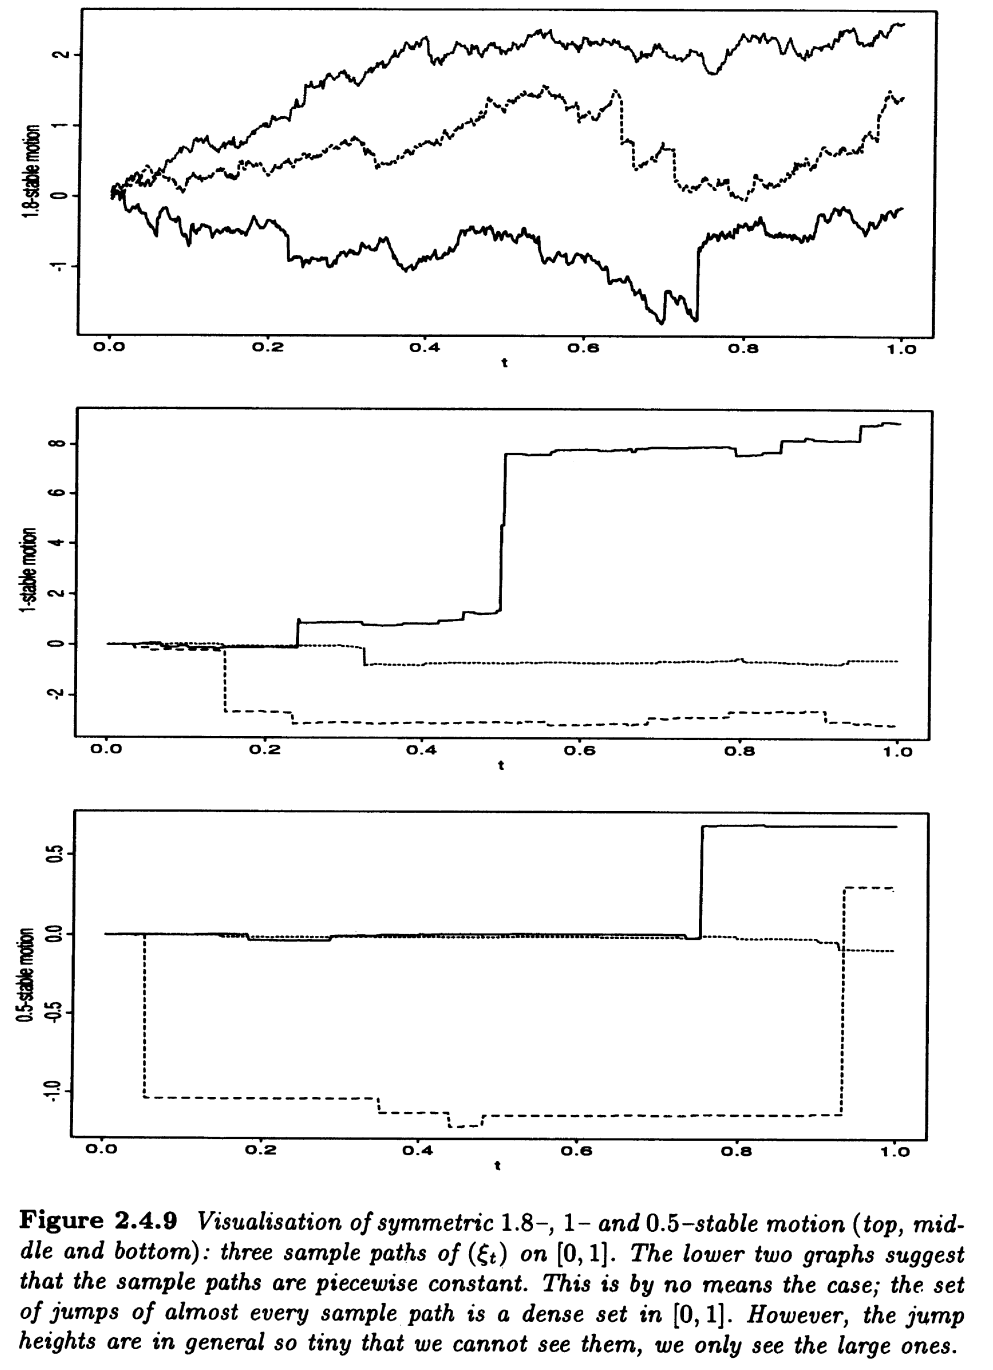
\includegraphics[height=0.50\textheight]{figures/e2-stable-process-path.png}
  \caption{$\alpha$-稳定过程的样本路径。图片来自 \cite{embrechts1997}, p.~94}
  \label{fig:e2:stable-process-path}
\end{figure}

关于平稳独立增量性，我们补充如下引理

\begin{lemma}[$\alpha$-稳定过程的增量分布]
\label{lem:ext-fclt:stable-increments}

设 $\xi(t)$ 是 $[0,1]$ 上的 α-稳定过程，则对 $0\le s<t\le 1$ 有
\[\xi(t) - \xi(s) \overset{\rm d}{=} (t-s)^{1/\alpha}\,\xi(1)\]
\end{lemma}

\begin{proof}

设 $\xi(t)$ 的特征函数为
\[\begin{aligned} \mathbb{E}[\exp\{i\lambda \xi(t)\}] = \exp\{-c(t) |\lambda|^\alpha (1 - i\beta \,\text{sign}(\lambda) z(\lambda,\alpha))\}\\ \end{aligned}\]
利用平稳独立增量，
\[\begin{aligned} \mathbb{E}[\exp\{i\lambda \xi(t)\}]  &= \mathbb{E}[\exp\{i\lambda \xi(s)\}]\, \mathbb{E}[\exp\{i\lambda (\xi(t) - \xi(s))\}] \\ &= \mathbb{E}[\exp\{i\lambda \xi(s)\}]\, \mathbb{E}[\exp\{i\lambda \xi(t-s)\} ]\\ &= \exp\{-(c(s) + c(t-s)) |\lambda|^\alpha (1 - i\beta \,\text{sign}(\lambda) z(\lambda,\alpha))\}, \end{aligned}\]
说明 $c(\cdot)$ 满足 $c(s)+c(t-s)=c(t)$、$c(0)=0$ 对 $0\le s<t\le 1$ 成立；这是一个经典的 \href{https://en.wikipedia.org/wiki/Cauchy\%27s_functional_equation}{Cauchy 方程} (Cauchy's functional equation)，其熟知的可测解为 $c(s) = c s$，其中 $c$ 为某个常数。由特征函数的性质可知 $c$ 必须为正。

因此
\[\mathbb{E}[\exp\{i\lambda (\xi(t) - \xi(s))\}] = \exp\{-c(t-s)|\lambda|^\alpha (1 - i\beta \,\text{sign}(\lambda) z(\lambda,\alpha))\}.\]
另一方面，$\xi(1)$ 的特征函数为 $\exp\{-c|\lambda|^\alpha (1 - i\beta \,\text{sign}(\lambda) z(\lambda,\alpha))\}$，从而
\[\mathbb{E}[\exp\{i\lambda (\xi(t) - \xi(s))\} ]= \mathbb{E}[\exp\{i\lambda (t-s)^{1/\alpha}\xi(1)\}]\]
由于特征函数唯一确定分布，故得
\[\xi(t) - \xi(s) \overset{\rm d}{=} (t-s)^{1/\alpha}\xi(1)\]
\end{proof}

由上述定理，我们可以得到 α-稳定过程的有限维分布表示：

\begin{corollary}\label{cor:ext-fclt:stable-finite-dimensional}
设 $0 = t_0 < t_1 < \dots < t_m \le 1$，则
\[(\xi(t_1), \xi(t_2), \dots, \xi(t_m)) \overset{\rm d}{=} \Bigl( t_1^{1/\alpha} Y_1,\; t_1^{1/\alpha} Y_1 + (t_2-t_1)^{1/\alpha} Y_2,\; \dots,\; \sum_{i=1}^m (t_i-t_{i-1})^{1/\alpha} Y_i \Bigr),\]
其中 $Y_1,\dots,Y_m$ 独立同分布，且 $Y_1 \overset{\rm d}{=} \xi(1)$。
\end{corollary}

\section{稳定泛函中心极限定理}

类似于 Donsker 定理，我们会问：\emph{是否每一个 α-稳定过程都可以作为某个部分和过程序列 }$S_n(\cdot)$* 的极限*？答案是肯定的，

\begin{theorem}[稳定泛函中心极限定理]
\label{thm:ext-fclt:stable-fclt}

设 $X_1, X_2, \dots$ i.i.d.，且属于某个位置参数 $\gamma=0$ 的非退化 α-稳定分布 $G_\alpha$ 的吸引域，即，存在缓变函数 $L(\cdot)$ 和中心化常数 $a_n$，使得
\[\frac{S_n - a_n}{n^{1/\alpha} L(n)} \overset{\rm d}\to Z_\alpha,\]
其中 $Z_\alpha$ 是服从 $G_\alpha$ 的随机变量。则，在 $\mathcal{D}[0,1]$ 空间中、配备 Skorokhod 度量 $d_0$ ，$[0,1]$ 上的随机过程
\[\xi^{(n)}(t) := \frac{1}{n^{1/\alpha} L(n)} \bigl( S_{[nt]} - a_{[nt]} \bigr)\]
弱收敛于一个 α-稳定过程 $\xi(t)$，且 $\xi(1) \overset{\rm d}{=} Z_\alpha$。

\end{theorem}

\begin{remark}

% \begin{itemize}
% \tightlist
% \item
  当 $\alpha=2$ 且 $\mathbb{E}[X_1^2] < \infty$ 时，$L(n)$ 可视为常数，且 $a_n = n\mathbb{E}[X_1]=n\mu$，定理退化为经典的 Donsker 定理。
% \item
%   吸引域条件等价于 $X_1$ 的分布函数 $F(x)$ 满足：存在缓变函数 $L_1(x)$，使得
%   \[
%   1-F(x) \sim c_+ x^{-\alpha} L_1(x),\qquad
%   F(-x) \sim c_- x^{-\alpha} L_1(x),qquad x\to\infty,
%   \]
%   其中 $c_+,c_-$ 非负，且 $c_+ + c_- > 0$。相关细节已经在
% \item
%   关于 $a_n$ ：对 $1< \alpha_n\le 2$ 都可以取 $a_n=n\mu$ 。当 $0<\alpha_n\le 1$ 时期望不存在，不过，例如 $X_1$ 的分布关于 0 对称时，则可取 $a_n=0$ 。
% \item
%   \emph{缓变函数 }(slow varying) $L(x)$ 指的是在无穷远处的缩放几乎不改变函数值： $\lim\limits_{x\to\infty} L(tx)/L(x)=1$ 对任意 $t>0$。常见例子：常函数、$\log x$、$\log \log x$ 等。
% \item
%   关于 GCLT 和吸引域更详细的内容请见 \hyperref[ext:stable-distributions]{扩展阅读《稳定分布》}。
% \end{itemize}
\end{remark}

对于稳定 FCLT，我们依然可以对其用连续映射定理，例如前文中关于 $f_1,f_2,f_3$ 函数的例子仍成立。

稳定 FCLT 有着更加广泛的应用：它可以用于模拟物理学中的超扩散 (superdiffusive) 行为、具有极端波动的金融数据，以及由非正态的 α-稳定噪声驱动的 SDE 的极限研究。%一个例子是随机梯度下降 (SGD) 的统计推断：

% \href{https://zhuanlan.zhihu.com/p/1988711005933549288}{当随机梯度没有有限方差时，我们还能做统计推断吗？}

\subsection{一个简单的模拟}

FCLT（Donsker 定理）和稳定 FCLT 不仅是一个理论结果，也提供了模拟 Brown 运动和 α-稳定过程的实用方法。例如：

\begin{itemize}
\tightlist
\item
  取 $n$ 足够大，生成 $X_1,\dots,X_n$ 独立同分布 $N(0,1)$，构造 $\widetilde S_n(t)$。得到的阶梯函数就是 Brown 运动的一个近似样本路径。
\item
  对于 α-稳定过程，可以生成独立同分布的 α-稳定随机变量 $Y_i$ ，然后构造 $\xi^{(n)}(t) = n^{-1/\alpha} \sum_{i=1}^{[nt]} Y_i$。当 $n$ 足够大时，其路径逼近真实 α-稳定过程。
\end{itemize}

如何生成独立同分布的 α-稳定随机变量？由于α-稳定分布（除少数特例外）没有显式的概率密度函数，如何高效生成其随机数曾是一个难题；目前最通用的方法是 \emph{\textbf{\href{https://en.wikipedia.org/wiki/Stable_distribution\#Simulation_of_stable_variates}{Chambers--Mallows--Stuck (CMS)}} } \textbf{\emph{算法}}，来自 \cite{chambers1976}。简而言之，取 $U\sim\mathcal U\left(-\tfrac\pi2,\tfrac\pi2\right)$ 服从均匀分布、 $E\sim\mathrm{Exp}(1)$ 服从指数分布，那么下式生成偏度系数 $\beta=0$ 、位置参数 $\gamma=0$ 、尺度参数 $c=1$ 的的标准 α-稳定分布
\[\frac{\sin(\alpha U)}{(\cos U)^{1/\alpha}}\left(\frac{\cos((1-\alpha)U)}{E}\right)^{(1-\alpha)/\alpha}\]
特别地 ，当 $\alpha=1$ 时，CMS 算法退化到生成标准 Cauchy 分布的 tan 变换 $\tan U\overset{\rm d}=\mathrm{Cauchy}(0,1)$ ；当 $\alpha=2$ 时，CMS 算法退化为 $2\sin U\sqrt{E}\overset{\rm d}=\mathcal N(0,2)$ ，再利用 $\mathrm{Exp}(1)\overset{\rm d}=-\ln (\mathcal U(0,1))$ 和 $\sin(\mathcal U(-\tfrac\pi2,\tfrac \pi2))\overset{\rm d}=\cos(2\pi\mathcal U(0,1))$ 可以得到
\[\mathcal N(0,1)\overset{\rm d}=\cos(2\pi U_1)\sqrt{-2\ln U_2},\quad  U_1,U_2\sim\mathcal U(0,1)\text{ i.i.d.}\]
这便是著名的 \href{https://en.wikipedia.org/wiki/Box\%E2\%80\%93Muller_transform}{Box--Muller 变换}。

我们写一个生成 α-稳定过程样本路径的 Mathematica 代码，固定 $n=1000$ ，

\begin{verbatim}
(* 固定参数 *)
α = 1.5;
n = 1000;
dt = 1/n;

SeedRandom[0];

(* 执行 CMS 算法生成 n 个样本 *)
U = RandomReal[{-π/2, π/2}, n];
Eexp = RandomReal[ExponentialDistribution[1], n];

inc = (dt^(1/α) Sin[U α] (Cos[U (1-α)]/Eexp)^((1-α)/α))/Cos[U]^(1/α);

(* 累积和得到路径 *)
path = Accumulate[inc];

(* 绘图 *)
ListPlot[path, DataRange -> {0, 1}, 
         PlotRange -> {{0, 1}, {-5, 5}}, 
         Joined -> If[α == 2, True, False], 
         ImageSize -> 500]
\end{verbatim}

上述程序的一次模拟结果如图~\ref{fig:e2:stable-process-simulation} 所示。

\begin{figure}[htbp]
  \centering
  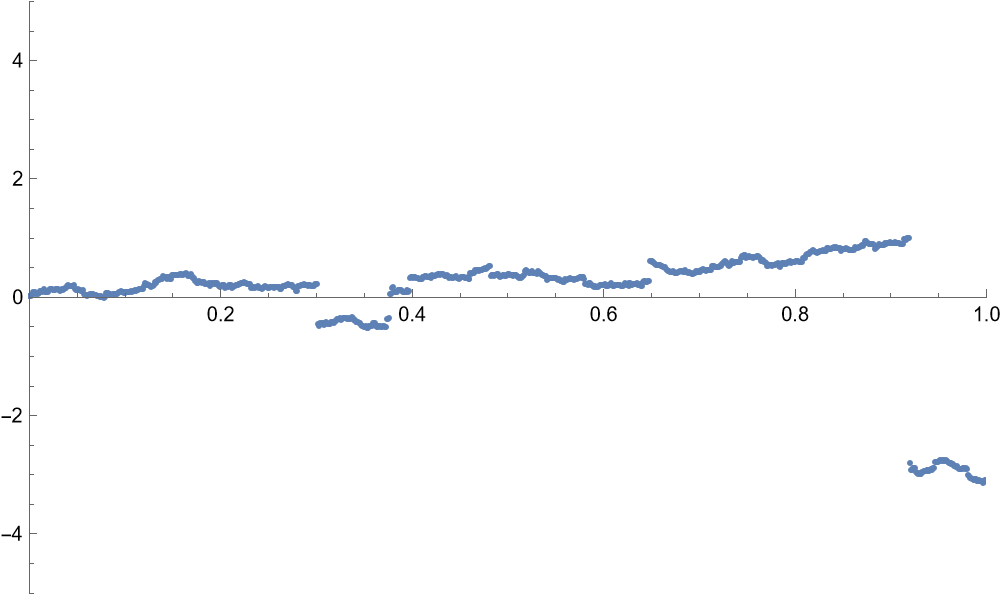
\includegraphics[width=0.88\textwidth]{figures/e2-stable-process-simulation.png}
  \caption{$\alpha$-稳定过程的模拟路径（Mathematica 13.3）}
  \label{fig:e2:stable-process-simulation}
\end{figure}

如果我们让 $\alpha$ 不断增加到 2，将看到 α-稳定过程的轨道越来越靠近连续，直至 $\alpha=2$ 时退化为 Brown 运动。可见 \href{https://demonstrations.wolfram.com/StableLevyProcess}{Wolfram Demonstrations Project}。


% \begin{figure}[htbp]
%   \centering
%   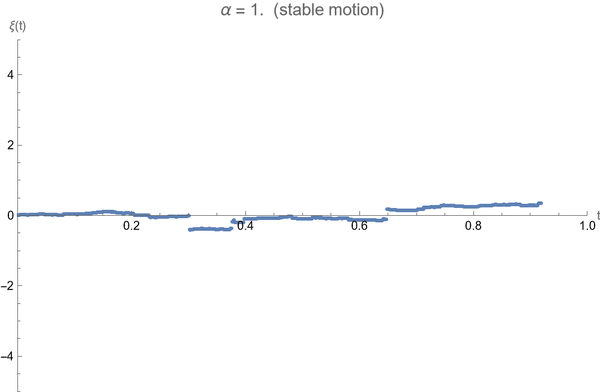
\includegraphics[width=0.88\textwidth]{figures/e2-stable-process-animation.png}
%   \caption{$\alpha$ 增加到 $2$ 时样本路径的变化；静态 PDF 展示原动画首帧（Mathematica 13.3）}
% \end{figure}

% 亦
